\newpage
\subsection{[U] Creating a list}
In order to create a list just click on the following button that is present on the right-side bar of the chat.

% Inserire immagine del bottone
\begin{figure}[H]
  \centering 
  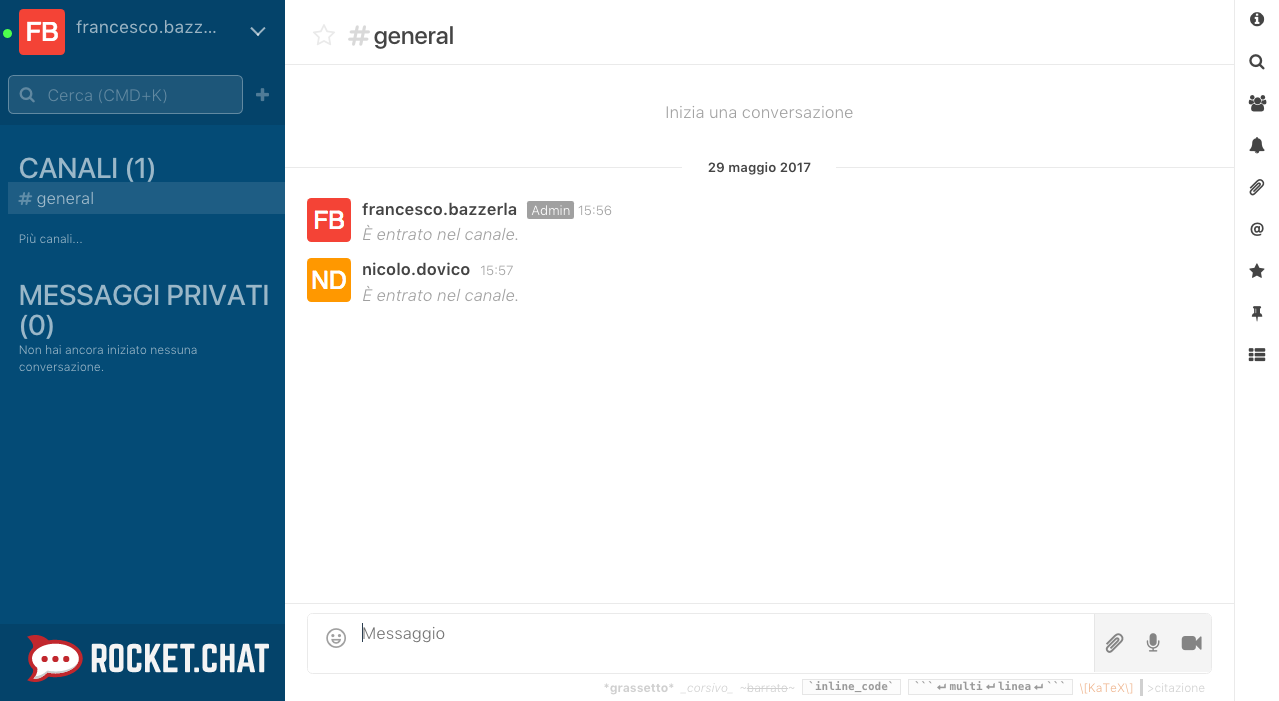
\includegraphics[width=\textwidth]{Sections/3-HowToUse/Images/channel_empty.png}
  \caption{Bubble creation button.}
\end{figure}

This will open the following screen, where you can input all the information that you want about the list, reminding that the only \textbf{required option} is the list's title.

\begin{figure}[H]
  \centering 
  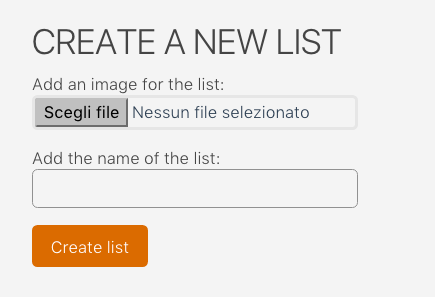
\includegraphics[width=\textwidth]{Sections/3-HowToUse/Images/list_create.png}
  \caption{Bubble creation button.}
\end{figure}

Once that all the information are input, in order to create the list just click on the \textit{"Create"} button, which will create the bubble as shown below.

\begin{figure}[H]
  \centering 
  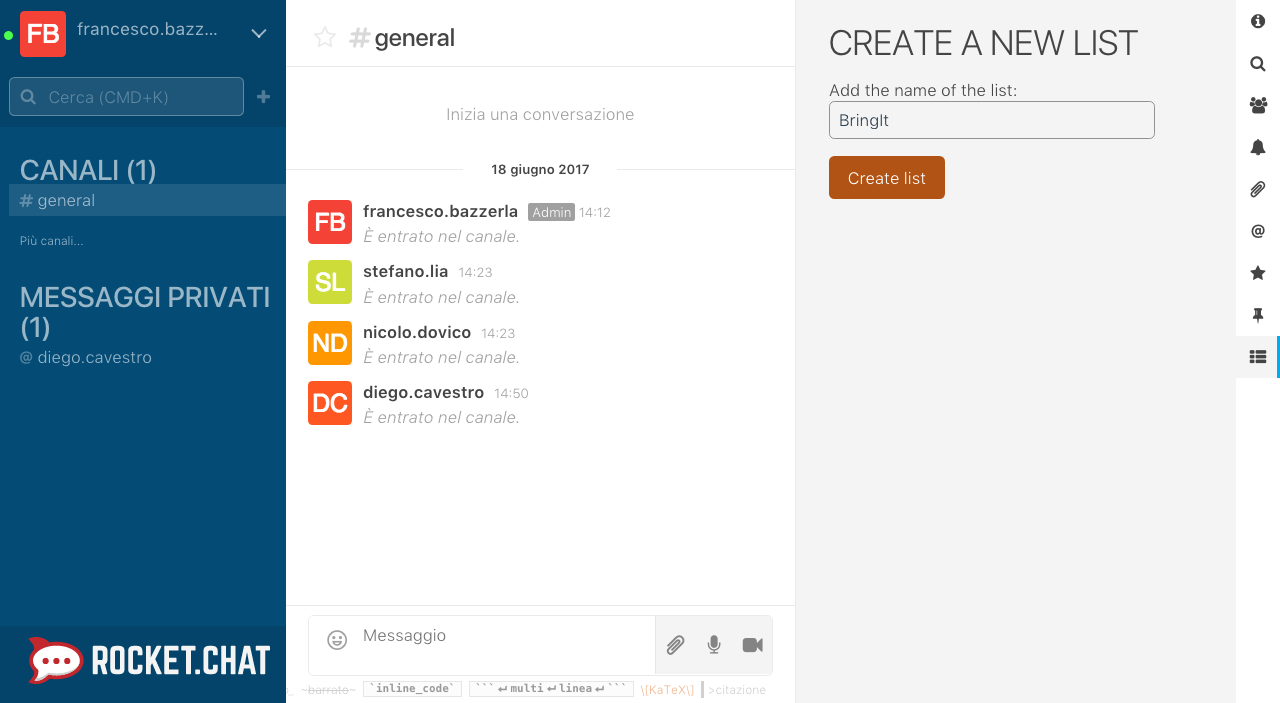
\includegraphics[width=\textwidth]{Sections/3-HowToUse/Images/list_create_filled.png}
  \caption{Bubble creation button.}
\end{figure}

% Inserire immagine della bolla creata
\begin{figure}[H]
  \centering 
  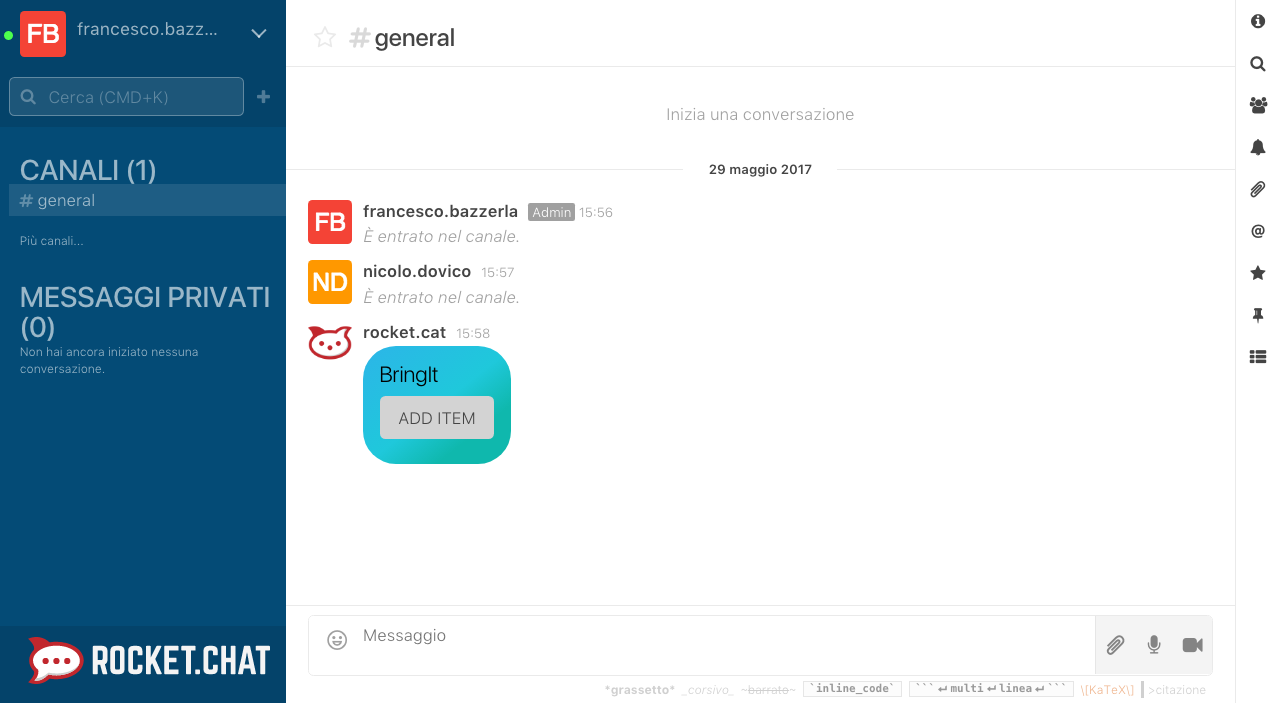
\includegraphics[width=\textwidth]{Sections/3-HowToUse/Images/bubble_empty.png}
  \caption{Created bubble which represents the list.}
\end{figure}